\chapter{Background}
	\section{Definition of terms}
		\subsection{Deep Zoom Image Format}
			The Deep Zoom Image Format (.dzi)\nmc{.dzi}{Deep Zoom Image Format} is an
			xml-based file format maintained by Microsoft\footnote{See
			https://msdn.microsoft.com/en-us/library/cc645077(v=vs.95).aspx for further
			details.} to improve performance and quality in the handling of large image
			files. Therefore an image will be represented in a tiled pyramid scheme (see
			fig. 2.1).
			
			\begin{figure}[!htbp]
				\begin{center}
					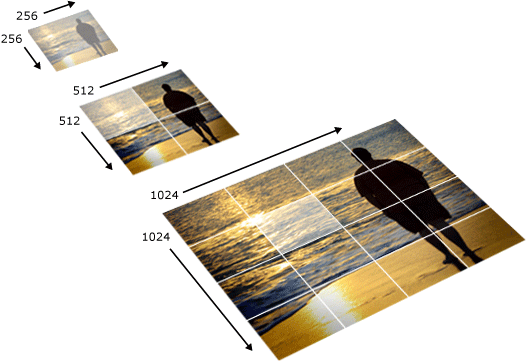
\includegraphics[scale=0.5]{img/dzi_pyramid.png}
					\caption{example of the dzi pyramid image representation (source:
					https://i-msdn.sec.s-msft.com/dynimg/IC141135.png)}
					\label{fig:abb2.1}
				\end{center}
			\end{figure}

			As seen in fig. 2.1 there are multiple versions of a single image in
			different resolutions. The idea behind this is, that if a user wants to see a
			whole picture zoomed out or as a small thumbnail, it is not necessary to
			load the image file in its highest resolution. To save bandwidth a version
			with a smaller resolution is loaded. If the user wishes to zoom in on a
			specific area of the image, a version with a higher resolution is loaded.
			Once again, however, it is not necessary to load the whole image, since only
			a fraction of it will be visible. For this reason there are tiles of the
			image which are loaded instead (see highlited tiles in fig. 2.1).
			
			Each resolution in the pyramid is called a \emph{level}. At each level the
			image is scaled down by the factor 4 (2 in each dimension). In other words, a
			level can be defined as an image with the resolution 2*level for height and
			width, resulting in a resolution of (2*level)*(2*level). Levels are counted
			from level 0 (1*1 Pixel). E.g. the levels shown in fig. 2.1 are:
			\begin{itemize}
			  \item level 8 ($2^8=256$) for the $256^2$ pixel image
			  \item level 9 ($2^9=512$) for the $512^2$ pixel image
			  \item level 10 ($2^10=1024$) for the $1024^2$ pixel image
			\end{itemize}

\subsection{Microservice}
\subsection{Machine Learning}
\subsection{Neural Networks}
\section{Process chain}
\subsection{Description}
\subsection{Definition of Conversion Service}
\subsection{Definition of Annotation Service}
\subsection{Definition of Tesselation Service}